% Section 1-6
\section{半导体器件基本方程}

半导体器件内的载流子在外场作用下的运动规律可以用一套基本方程来加以描述,
是分析一切半导体器件的基本数学工具,
由三组方程所组成:麦克斯韦方程组、输运方程组和连续性方程组。

\subsection{泊松方程}
泊松方程原始形式:
\begin{equation}
    \nabla \cdot \boldsymbol{D} = \rho_V(x,y,z)
\end{equation}
其中 $\boldsymbol{D}$ 代表电位移矢量;$\rho_V(x,y,z)$ 代表自由电荷的体密度。

在半导体中,$\rho_V=q(p-n+N_D-N_A)$;
静态或低频下,$\boldsymbol{D}=\varepsilon_s\boldsymbol{E}$ 代表半导体的电容率,
$\boldsymbol{E}$ 代表电场强度矢量,再考虑到 $\nabla \psi = -\boldsymbol{E}$,
得到:
\begin{equation}
    \nabla \cdot \boldsymbol{E} = -\nabla^2\psi
    = {q \over \varepsilon_s}(p-n+N_D-N_A)
\end{equation}
其中,$\psi$ 代表静电势,$q$ 代表一个电子所带电荷量的绝对值,
$p$、$n$、$N_D$、$N_A$ 分别代表空穴、电子、电离施主杂质和电离受主杂质的浓度。

泊松方程表明:空间任意点的电位移(或电场强度)矢量的散度正比于该点的电荷密度。

物理意义:电感线总是出发于正电荷而终止于等量的负电荷。

\subsection{输运方程}

又称为电流密度方程:
\begin{align}
\boldsymbol{J}_n &= q\mu_nn\boldsymbol{E} + qD_n\nabla{}n \\
\boldsymbol{J}_p &= q\mu_pp\boldsymbol{E} - qD_p\nabla{}p
\end{align}
其中,$\boldsymbol{J}_n$、$\boldsymbol{J}_p$
分别是电子电流密度矢量和空穴电流密度矢量,
$D_n$、$D_p$ 分别代表电子和空穴的扩散系数,
$\mu_n$、$\mu_p$ 分别代表电子和空穴的迁移率。

未完待续...

\subsection{电路}
由电阻器、电容器、线圈、变压器、晶体管、运算放大器、传输线、电池、发电机和信号发生器等
电器器件和设备连接而成的电路,称为实际电路。
根据实际电路的集合尺寸($d$)与其工作信号波长($\lambda$)的关系,可以将它们分为两大类:
满足 $d\ll\lambda$ 条件的电路称为集总参数电路,
其特点是电路中任意两个端点间的电压和流入任一器件端钮的电流是完全确定的,
与器件的几何尺寸和空间位置无关。不满足 $d\ll\lambda$ 条件的另一类电路称为分布参数电路。
本书只讨论集总参数电路,今后简称为电路。

\subsection{电路模型}
研究集总参数电路特性的一种方法是用电器仪表对实际电路直接进行测量。
更重要的一种方法是将实际电路抽象为电路模型,用电路理论的方法分析计算出电路的电气特性。
对于集总参数电路,当不关心器件内部的情况,只关心器件端钮上的电压和电流时,
可以定义一些理想化的电路元件来近似模拟器件端钮上的电气特性。
定义电阻元件是一种只吸收电能(可以转换为其他形式的能量)的元件,
电容元件是一种只存储电场能量的元件,
电感元件是一种只存储磁场能量的元件。
在电路分析中,为了便于看出电路模型中各元件的连接关系,
常采用仅仅表示元件连接关系的拓扑结构图。

图 \ref{fig:fig1_1_1} 列举了本书采用的部分电路元件的图形符号\footnote{由于时间紧迫,先拍照借图}。

\begin{figure}[htbp]
\centering
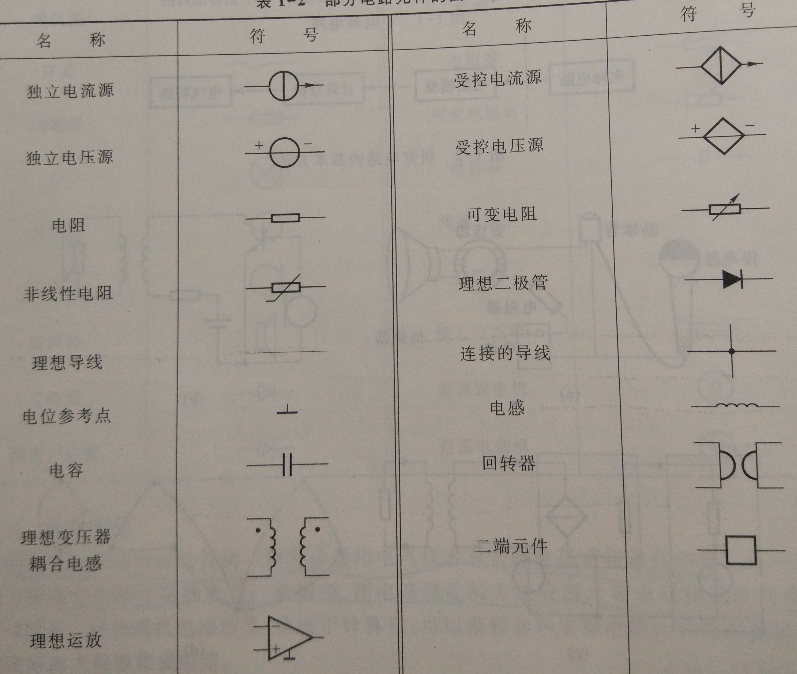
\includegraphics[scale=0.4]{s1-1-g.png}
\caption{部分电路元件的图形符号}\label{fig:fig1_1_1}
\end{figure}

电路模型近似地描述实际电路的电气特性。
根据实际电路的不同工作条件以及对模型精确度的不同要求,
应当用不同的电路模型模拟同一实际电路。

本课程的主要任务是研究电路模型(简称为电路)的各种分析方法,
其目的是通过对电路的分析研究来预测实际电路的电气特性,
以便指导改进实际电路的电气特性和设计制造出新的实际电路。
电路的研究问题可以分为两类。
一类是电路分析:已知电路结构和元件特性,分析电路的特性;
另一类是网络综合:根据电路特性的要求来设计电路的结构和元件参数。
本课程是电路的入门课程,主要讨论电路分析问题,也给出一些电路设计的例题。

今后,“电路”可能指实际电路,也可能指实际电路的电路模型。
